\documentclass{article}
\usepackage[margin=1in]{geometry} 
\usepackage{amsmath,amsthm,amssymb,amsfonts, bm, fancyhdr, color, comment, graphicx, environ, tikz}
\usepackage{pgfplots}
\pgfplotsset{compat=1.15}
\usepackage{mathrsfs}
\usetikzlibrary{arrows}
\pagestyle{empty}
\usepackage{xcolor}
\usepackage{mdframed}
\usepackage[shortlabels]{enumitem}
\usepackage{indentfirst}
\usepackage{hyperref}
\hypersetup{
    colorlinks=true,
    linkcolor=blue,
    filecolor=magenta,      
    urlcolor=blue,
}


\pagestyle{fancy}


\newcommand{\Li}{\text{Li}}
\title{\textbf{Final Exam}}
\rhead{CMSC828V} 
\author{Sriram Balasubramanian}


\begin{document}
 \maketitle

For the questions with a coding component, please refer to the Jupyter notebook in \href{https://github.com/SriramB-98/CMSC828V-projects/tree/main/FinalExam}{this Github repository}
. 


\begin{enumerate}


\item Downloaded, see accompanying code.

\item After running DFS on the graph, we find that there is only 1 connected component with 7624 nodes in the graph. 

\begin{figure}
\centering
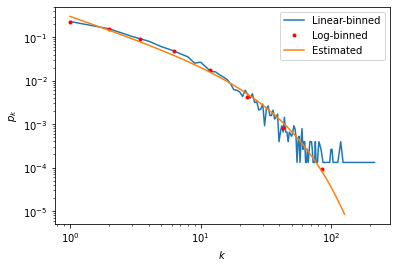
\includegraphics[scale=0.5]{pk_vs_k.png}
\caption{Degree distribution $p_k$ vs $k$ using linear binning, log binning and estimating parameters using least squares}
\label{fig:pk_vs_k}
\end{figure}

\item The degree distribution is plotted using linear binning and log binning in Figure \ref{fig:pk_vs_k}. The exact values of $p_k$ for each $k$ can be found in the Jupyter notebook

\item We fit the log-binned data to the form $p_k = Ce^{-\alpha k}k^{-\tau}$.

  Taking $\log$ on both sides and rearranging, we have $\log p_k = \log C -\alpha k -\tau \log k$. Using a linear least squares solver to solve for $C, \alpha, $ and $\tau$, we get $C = 0.3014, \alpha=0.0457, \tau = 0.9837$.
  
  The estimated $p_k$ vs $k$ curve is plotted in Figure \ref{fig:pk_vs_k}

\item Using the \texttt{average\_shortest\_path\_length} from the \texttt{networkx} package in Python, we can compute the average shortest path length in the actual network as 5.232 .

From \cite{newman}, we obtain the expression of the average shortest path length $\ell$ as 

$$ \ell = \frac{\ln [ (N-1)(z_2 - z_1) + z_1^2 ] -  \ln z_1^2}{\ln z_2/z_1} \approx 1 + \frac{\ln N - \ln z_1}{\ln z_2 - \ln z_1}$$

where $z_1$ is the average number of nearest neighbors (or the average degree), and $z_2$ is the average number of second nearest neighbors. Using generating functions, we obtain $z_1 = G_0'(1)$ and $z_2 = G_0'(G_1(1))G_1'(1) = G_0'(1)G_1'(1) $ where $G_0$ and $G_1$ are the generating functions for the degree distribution and excess degree distribution respectively. 

For the exponential power cut-off random graph, we have the following equations from \cite{newman}
\begin{align}
z_1 &= \frac{\Li_{\tau - 1}(e^{-\alpha})}{\Li_{\tau }(e^{-\alpha})} \\
z_2 &= \frac{\Li_{\tau - 2}(e^{-\alpha})-\Li_{\tau - 1}(e^{-\alpha})}{\Li_{\tau }(e^{-\alpha})}\\
\end{align}

where $\Li_s(z) = \sum_{k=1}^\infty \frac{z^k}{k^s}$ is the polylogarithm function.  

Using the estimated values of $\alpha$ and $\tau$ for computing $z_1$ and $z_2$ and plugging it into the equation for $\ell$, we get $\ell \approx 3.2551$

\item The clustering coefficient for the actual network is estimated to be $\approx 0.1786$

We can calculate the clustering coefficient for the random graph with same degree distribution as follows. 

Let $v$ be an arbitrary node of degree 2 or more. We randomly pick two of its first neighbors $i$ and $j$ with excess degrees $k_i$ and $k_j$ . The probability that there is a link between $i$ and $j$ is $$\frac{k_i k_j}{nz}$$
where $n$ is the total number of nodes and $z = \langle k \rangle$ is the average node degree.

Then assuming that $k_i$ and $k_j$ are independent, $$ C_{random} = E_{k_i, k_j \sim Q(k)}\left[\frac{k_i k_j}{nz}\right] = \frac{ E_{k \sim Q(k)}[k]^2 }{n \langle k \rangle}$$ where $Q(k)$ is the excess degree distribution. Now, $$ E_{k \sim Q(k)}[k] = \sum_{k=0}^\infty kq_k = \frac{1}{z} \sum_{k=0}^\infty k(k+1)p_{k+1} = \frac{1}{z} \sum_{k=0}^\infty k^2 p_{k} - k p_k = \frac{\langle k^2 \rangle - \langle k \rangle}{\langle k \rangle} $$

Plugging this into the formula for $C_{random}$, we get $$C_{random} = \frac{[\langle k^2 \rangle - \langle k \rangle]^2}{n\langle k \rangle^3} = \frac{z_2^2}{n z_1^3}$$

Using the values of $z_1$ and $z_2$ from the previous question, we get $C_{random} \approx 0.0088$

\item The actual graph shows characteristics of small-world networks, which typically have a ``small" average shortest path lengths scaling as $\log N$ where $N$ is the total number of nodes, and high clustering coefficient as compared to chance. The random graph, however, has a small clustering coefficient. In fact, as $N$ approaches $\infty$, the clustering coefficient for the random graph approaches $0$. 

The clustering coefficient for the random graph is much lower than that of the actual graph. This is because the parameters of the probability distribution we estimated from the log-binned data predict much lower high degree nodes, or hubs, than are actually found in the graph, as can be seen in \ref{fig:pk_vs_k} where the actual distribution has a much fatter tail as compared to the random graph. These hubs contribute disproportionately to the clustering coefficient. Since the model predicts lower number of hubs, it also predicts low clustering coefficient.

The average shortest path length for the random graph is also lower that that of the actual graph. While the clustering coefficient of the random graph is indeed much lower than the clustering coefficient of the actual network, there exist quite a few more nodes with only 1 neighbour as compared to what the model predicts. This means that distance between these nodes and the rest are higher than what the model predicts, which implies that average shortest path length is higher than the prediction by the model. 

\item We know that $$T_c = \frac{G_0'(1)}{G_0''(1)} = \frac{\langle k \rangle }{\langle k^2 \rangle - \langle k \rangle }$$

Using empirical estimates for  $\langle k^2 \rangle \approx 185.437$ and $\langle k \rangle \approx 7.294$, we get $T_c \approx 0.041$

\item We run the SIR model for 20 timesteps 10 times with $T=0.4$, and plot the number of sick nodes at each time step for all 10 runs in Figure \ref{fig:random_SIR_runs}

\begin{figure}
\centering
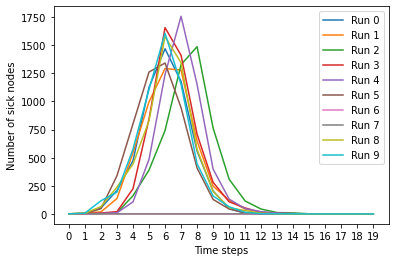
\includegraphics[scale=0.5]{random_SIR_runs.png}
\caption{10 random runs of the SIR model}
\label{fig:random_SIR_runs}

\end{figure}

We observe an epidemic in 8 runs. Whenever an epidemic is observed, around 25 - 29\% of nodes are infected at the peak of the epidemic. The exact fractions for each of the 10 runs are 

$0.699, 0.703, 0.7053, 0.7003, 0.7042, 0.6999, 0.0004, 0.0005, 0.7046, 0.7148$. 

The mean and standard deviation of the fraction of affected nodes during epidemics is 0.704 and 0.0046


\item 

\begin{enumerate}
\item The critical transmissibility $T_c = \frac{G_0'(1)}{G_0''(1)} = \frac{z_1}{z_2} \approx 0.0461$

\item We solve the following equations to get the fraction of nodes infected  as a function of transmissibility $S(T)$ (fraction of nodes in the giant component in the transmissibility graph)

\begin{align}
H_1(1, T) &= G_1(H_1(1, T), T) \\
H_0(1, T) &= G_0(H_1(1, T), T) \\
S(T) &= 1 - H_0(1, T)\\
\end{align}

We first solve $h = G_1(h, T) = G_1(1 + (h-1)T)$. From \cite{newman}, we know that $G_1(x) = \frac{\Li_{\tau -1}(xe^{-\alpha})}{x\Li_{\tau -1}(e^{-\alpha})}$. Therefore, we solve the following equation:

$$ h = \frac{\Li_{\tau -1}((1 + (h-1)T)e^{-\alpha})}{(1 + (h-1)T)\Li_{\tau -1}(e^{-\alpha})}$$

Since we only need to know $S(0.4)$, we substitute $T=0.4$ and solve the equation numerically to get $h \approx 0.1128$

Now, $S(0.4) = 1 - G_0(h, 0.4) = 1 - G_0(1 + 0.4(h-1))$. We have $G_0(x) = \frac{\Li_{\tau}(xe^{-\alpha})}{\Li_{\tau}(e^{-\alpha})}$. Substituting the value of $h$, we get $S(0.4) = 1 - G_0(1 + 0.4(0.11) ) \approx  0.6962$.

\item Suppose that a fraction of nodes $p$ is randomly removed from the transmission graph. From \cite{cohen}, we know that ${G^*}_0(x, p, T) = G_0(1 + (1-p)(x-1), T )$ where ${G^*}_0(x)$ is the new generating function after removing the nodes. But $G_0(x, T) = G_0(1 + (x-1)T)$, therefore, ${G^*}_0(x, p, T) = G_0(1 + (1-p)T(x-1))$. 
The criterion for this new graph to have a giant component is $(1-p)T \geq \frac{G_0'(1)}{G_0''(1)} \approx 0.0457$. Therefore, $1-p \geq 0.0461/0.4 = 0.11525$, or $p \leq 0.88475 = p_c$ If more than $p_c$ fraction of nodes are removed (in this case vaccinated), the graph no longer has a giant component and there will not be an epidemic.

\end{enumerate}

The critical transmissibility of the actual graph is 0.041 which is slightly lower than the theoretical estimate 0.0461. Also, the theoretical estimate of the fraction of nodes affected by the epidemic which is around 0.6962 is slightly smaller than the fractions observed in the 10 runs in Figure \ref{fig:random_SIR_runs}. 

Critical transmissibility and fraction of affected nodes are inversely proportional. The higher the critical transmissibilty, the lower the fraction of affected nodes at $T=0.4$, or any fixed $T$. If the critical transmissibility is greater than 0.4, we do not observe epidemics and fraction affected is close to 0. This relationship is true for both the actual and the random graph.

\end{enumerate}

\begin{thebibliography}{2}

\bibitem{newman} M. E. J. Newman, S. H. Strogatz, and D. J. Watts, 2001, Random graphs with arbitrary degree distributions and their applications

\bibitem{cohen} Reuven Cohen, Keren Erez, Daniel ben-Avraham, and Shlomo Havlin, 2000, Resilience of the Internet to Random Breakdowns

\end{thebibliography}


\end{document}